\chapter{Attitude control}
\section{Modelling}
This section provides a description of the dynamic and kinematic equations of motion which constitute the basis for further analysis and description of the forces and/or disturbances, which may affect a rigid body within LEO. The coordinate systems are defined first and then the model for the satellite is derived, based on rigid body dynamics and kinematics. 
%In order to control the distance between two or more satellites in orbit, a mathematical description of the governing equations should be derived. Since precious work have been made in previous projects, and all the measurements are available, in-depth analysis it is deemed not necessary. 
%
\subsection{Kinematics}
This section will provide the orbit-attitude determination of the satellite using quaternion representation. Since the differential drag control method is based on the rotation of the satellite in order to achieve the effective cross-sectional area, a notation with respect the collaborating frames have been obtained.

Quaternion parameterization it is deemed useful for the kinematic analysis of the satellite. Since the product of two quaternions gives the combined rotation, we shall specify the representation of rotation at time $t$ of the collaborating frames in order to derive the combined rotation at time $t+\Delta{t}$. The orientation of the rigid body at time $t$ is represented as $q(t)$ and at time $q(t+\Delta{t})$ is the resulting quaternion at time $t+\Delta{t}$. The orientation of the controller reference frame $\hat{x_{c}}, \hat{y_{c}}, \hat{z_{c}}$ at time $\Delta{t}$ with respect the orientation at time $t$ can be represented as $q_{c}(\Delta_{t}$, then the orientation of the satellite at $t+\Delta{t}$ can found as
%
\begin{flalign}
	q(t+\Delta{t}) = {q_{c}(\Delta_{t}) \otimes q(t)}
	\label{eq:quaternionproduct}
\end{flalign}
%
with the components of the rotation axis unit vector along $\hat{x_{c}}, \hat{y_{c}}, \hat{z_{c}}$ at time $t$ \cite{SADC} written as $[e_{x} e_{y} e_{z}]$ respectively and $\Delta{\Phi}$ the rotation at time $\Delta(t)$, the parameters of the controller quaternion can be written\cite{SADC} as 
%
\begin{flalign}
	q_{1c} = {e_{x}\sin\frac{\Delta\Phi}{2}}
	\label{eq:controllerquaternion1}
\end{flalign}
%
\begin{flalign}
	q_{2c} = {e_{y}\sin\frac{\Delta\Phi}{2}}
	\label{eq:controllerquaternion2}
\end{flalign}
%
\begin{flalign}
	q_{3c} = {e_{z}\sin\frac{\Delta\Phi}{2}}
	\label{eq:controllerquaternion3}
\end{flalign}
%
\begin{flalign}
	q_{4c} = {\cos\frac{\Delta\Phi}{2}}
	\label{eq:controllerquaternion4}
\end{flalign}
%
combining the  \eqref{eq:controllerquaternion1} - \eqref{eq:controllerquaternion4} with \eqref{eq:quaternionproduct} we obtain 
%
\begin{flalign}
	q(t+\Delta{t})
	= 
	\left\{\cos\frac{\Delta\Phi}{2} I_{(4x4)}+\sin\frac{\Delta\Phi}{2}
	\begin{bmatrix}
		0 &e_{z}&-e_{y}&e_{x} \\
		-e_{z}&0&e_{x}&e_{y}  \\ 
		e_{y}&-e_{x}&0&e_{z} \\
		-e_{x} &e_{y}&-e_{z}&0
	\end{bmatrix} 
\right \} q(t)
	\label{eq:quaternionmult}
\end{flalign}  
%
where I is the $4x4$ identity matrix. Using the small angle approximation \cite{SADC} for infinitesimal $\Delta(t)$ and denoted $\omega$ the instantaneous change in angular velocity it is obtained 
%
 \begin{flalign}
 	q(t+\Delta{t}) = \left[1 + \frac{1}{2} \Omega \Delta(t)\right]q(t)
 	\label{eq:controllerquaternionfinal}
 \end{flalign} 
with $\Omega$ be the skew symmetric matrix\cite{SADC} 
\begin{flalign}
	\Omega
	= 
	\begin{bmatrix}
		0& \omega_{z}& - \omega_{y}& \omega_{x} \\
		-\omega_{z}& 0&\omega_{1}& \omega_{x}  \\ 
		\omega_{y}& -\omega_{x}&0& \omega_{z} \\
		-\omega_{x}& -\omega_{y}& -\omega_{z}&0
	\end{bmatrix} 
	\label{eq:skewsymmetricmatrixquaternion}
\end{flalign}
%
the angle approximations where taken as $\cos\frac{\Delta\Phi}{2} \simeq 1$ and $\sin\frac{\Delta\Phi}{2}\simeq \frac{1}{2} \omega \Delta(t) $
%
\subsection{Dynamic Model}
In order to describe the behavior of the satellite a dynamic model based on reaction wheels and by using Euler's equation of motion has been derived.   
%
Euler's equation of motion describing the rotation of a rigid body relates the time derivative of angular momentum to the applied torques\cite{SADC} and is given by: 
% 
\begin{flalign}
	\dot{L} = {N_{tot}- \omega }{\times {L}}
	\label{eq:eulerequation}
\end{flalign}
% 
where $N_{tot}$ represents all the external torques caused from the actuator and the disturbances, $\omega$ is the angular velocity of the satellite and $L$ is the total angular momentum of the satellite including reaction wheels, given by\cite{SADC}:
%
\begin{flalign}
	{L} = {I_{s}}{\omega}+{h_{tot}}
	\label{eq:angularmomentum}
\end{flalign}
%
where $h_{tot}$ is the vector of the angular momentum of the wheels $[h_1 \ h_2 \ h_3]^{T}$, all seen in the satellites coordinate system and $I_{s}$ is the inertia matrix of the satellite.
%
Inserting the equation \eqref{eq:angularmomentum} into \eqref{eq:eulerequation} we obtain
%
\begin{flalign}
	{\frac{d}{dt}(I_{s}{\omega})+\dot{h}_{(tot)}} ={N_{tot}-\omega}     {\times  ({I_{s}}{\omega} +{h_{tot}})}
	\label{eq:angularmomentum2}
\end{flalign}
For three reaction wheels attached at the body coordinate system which are the axis roll, pitch and yaw, three equations shall be derived. The derivation of the three equations of motion along with the diagonal inertia matrix can be found in the \appref{chap:A}.
%
For the ease of notation, the cross product can be written as matrix operation using the $S()$ representing the skew symmetric matrix. Solving for $\dot{\omega}$ the dynamic equation can be written as 
%
\begin{flalign}
	{\dot{\omega}}={-I_{s}^{-1}S(\omega)I_{s}^{-1}\omega-I_{s}^{-1}S(\omega)h_{tot}-I_{s}^{-1}\dot{h}_{(tot)}+I_{s}^{-1}N_{tot}}
	\label{eq:angularmomentum3}
\end{flalign} 
%
The rate of change in angular momentum $\dot{h}_{(tot)}$ can be absorbed from the controller. This can be written as:
%
\begin{flalign}
	{\dot{h}_{(mv)}} ={-N{mw}}
	\label{eq:rate of change}
\end{flalign}
%
where the negative sign denotes the absorbed momentum. The total torque from external disturbances can be written as $N_{dis}$. Rearranging, equation \eqref{eq:angularmomentum3} now reads 
%
\begin{flalign}
	{\dot{\omega}(t)} ={-I_{s}^{-1}S(\omega)I_{s}\omega(t)-I_{s}^{-1}S(\omega)h_{tot}+I_{s}^{-1}N_{c}(t)+I_{s}^{-1}N_{dis}(t)}
	\label{eq:angularmomentum4}
\end{flalign}
%
which constitute the dynamics of the satellite with three reaction wheels. At the final equation \eqref{eq:angularmomentum4} is shown the time dependency of the variables. 
\subsection{Equation of motion} \label{subsec:eom} 
The behaviour of the satellite attitude is described by the dynamic and kinematic equations, which give a non-linear state space representations.
\begin{flalign}
\begin{bmatrix}
	\vec{\dot q(t)} \\
	\vec{\dot \omega{(t)}}
\end{bmatrix} 	
= 
\begin{bmatrix}
	\frac{1}{2} \underline{\Omega}_{(4\times4)} \vec q(t) \\
	{-\underline{I}_{s}^{-1}\underline{S}(\vec{\omega})\underline{I}_{s}\vec{\omega}(t)-\underline{I}_{s}^{-1}\underline{S}(\vec{\omega})\vec{h_{mw}}+\underline{I}_{s}^{-1}\vec{N_{c}}(t)+\underline{I}_{s}^{-1}\vec{N_{dis}}(t)}
\end{bmatrix} 
	\label{eq:le}
\end{flalign}
where,\\
  $\vec{\dot q(t)} = [q_1 \ q_2 \ q_3 \ q_4]^T$ \\
  $\vec{\dot \omega{(t)}} = [ \omega_1 \ \omega_2 \ \omega_3]^T$ \\
  $\underline{\Omega}(\omega)$ is the $4\times4$ skew symmetric matrix \\
  $\underline{I}_{s}$ is the inertia matrix \\
  $\underline{S}(\omega)$ is the $3\times3$ skew symmetric matrix \\
  $\vec{N_{dis}}(t)$ is the disturbance torque \\
  $\vec{N_{c}}(t)$ is the control torque and is equal with $\vec{N_{mt}-N_{mw}}$, where $\vec{N_{mt}}$ is the torque from magnetorques and $\vec{N_{mw}}$ is the torque from momentum wheels \\
  
 %add underline and vec, h_tot -> h_mw; add the equation for dot(h_mw)
\subsection{Linearized equation of motion} \label{subsec:lem} 
The kinematic and dynamic equations are linearized around the operating point for the purpose of designing a linear controller. The quaternion $\vec{q(t)}$ is split in the operating point ($\vec{\bar{q}}$) and the error quaternion ($\vec{\tilde{q}}$) and the angular velocity $\vec{\omega}$ is split in the nominal value $\vec{\tilde{\omega}}$ and the error $\vec{\tilde{\omega}}$.
\begin{flalign}
	&\vec{q} = \vec{\bar{q}} \otimes \vec{\tilde{q}} \\
	&\vec{\tilde{q}} = \vec{\bar{q}}^{-1} \otimes \vec{q} \\
	&\vec{\omega} = \vec{\bar{\omega}} + \vec{\tilde{\omega}} 
\end{flalign}
	 Thus, the linearized equation of motion for the satellite are given by: 

\begin{flalign}
	\begin{bmatrix}
		\vec{ \dot {\tilde{q}}(t) } \\
	{ \dot {\tilde{\omega}}(t) }
	\end{bmatrix} 	
	= 
	\begin{bmatrix}
	-S(\bar{\omega}) &	\frac{1}{2} \underline{\vec 1}_{(3\times3)} \\
	 \underline{\vec 0}_{(3\times3)} &	{I_{s}^{-1}S(\omega)I_{s}\omega(t)-I_{s}^{-1}S(\omega)h_{tot}}
	\end{bmatrix} 
		\begin{bmatrix}
		\vec{  {\tilde{q}}(t) } \\
		{  {\tilde{\omega}}(t) }
    	\end{bmatrix} 	
+
	\begin{bmatrix}
	\underline{\vec 0}_{(3\times3)} \\
		{I_{s}^{-1}}
    \end{bmatrix} 	
  \tilde N_c(t)
	\label{eq:le}
\end{flalign}

\section{Disturbance Models}\label{sec:csf} 
\subsection{Gravity-Gradient torque}
An unbalanced satellite in orbit is subjected to a torque due to earth's non-uniform gravitational field . Assumed that the earth is a point mass and the satellite is a rigid body, the gravitational torque can be estimated. Each infinitesimal element of the satellite of mass \textit{$dm_i$} is subjected to an infinitesimal force \textit{$dF_i$} acting on the mass element located at position $R{i}$ from the earth's geometric centre that can be calculated as\cite{wertz}
\begin{flalign}
d\vec{F_i} = -G\frac{m_{earth}}{R_i^3}dm_i \cdot \vec{R_i}
	\label{eq:ref1}
\end{flalign}
where $G$ is the gravitational constant, $m_{earth}$ is the mass of the earth and $\vec{R_i}$ is the vector from the Earth's geometric centre to the infinitesimal element of the satellite. 

The torque about the geometric centre of the satellite due to a force \textit{$dF_i$} at a distance $r_i$ from the geometric centre of the satellite is calculated as:
\begin{flalign}
	d\vec{N_{gra}} =  r_i \times d\vec{F_i} 
	\label{eq:ref2}
\end{flalign}
 $r_i$ can be written as the sum of two vectors,$r_{co}$ which is the vector from geometric centre of the satellite to the centre of mass, and $r_{ci}$ which is the vector from the centre of mass to the infinitesimal element.  Therefore, the expression of the gravity gradient torque is obtained by integrating \eqref{eq:ref2} and thus we obtain\cite{wertz}
\begin{flalign}
	N_{gra} &= \int_{sat} (r_{co} +r_{ci}) \times d\vec{F_i}  
	\label{eq:ref3}
\end{flalign}
The vector $\vec{R_i}$ can be written as $\vec{R_i} = \vec{R_{sc}} + \vec{r_i}$. Finally assuming that the geometric centre of the satellite is aligned with its centre of mass, this is equal by setting $r_{co} = 0$, and by using the inertia matrix $I$, and replacing the term $dF_i$ by \eqref{eq:ref1}  the gravity gradient torque can be written as\cite{wertz}  
%
\begin{flalign}
N_{gra} &= \dfrac{3\mu}{R_{sc}^3}[\vec{\hat{R_{sc}}}\times(\vec{I} \vec{\hat{R_{sc}}})] 
\label{eq:ref4}
\end{flalign}
where $q_{i,s}$ is the quaternion that represents the rotation of the satellite in the inertia frame and $\otimes$ is the quaternion multiplication. Thus, the moment of force can be calculated by this expression above.
\subsection{Solar radiation}
The surface of the CubeSat will absorb or reflect the solar radiation, nevertheless, these two situations will alter the CubeSat, which will produce a torque about the satellite centre of mass(CoM). \cite{SADC}
The torque around CoM is given by:
\begin{flalign}
	N_{rad} = F_{rad} \times R_{CoM}
	\label{eq:tor}
\end{flalign}
where $F_{rad}$  is the solar radiation  and $R_{CoM}$ is the vector from the centre of mass to the geometric centre of radiation

The solar radiation $F_{rad}$ can be expressed as:
\begin{flalign}
	F_{rad} = C_{a} P A
	\label{eq:Pres}
\end{flalign}
where $C_{a}$ is the surface’s reflectance: 0 for a perfect absorber, 1 for a perfect reflector,   while $P$ is the solar flux and  $A$ is the radiated area

The solar flux can be computed as follows:
\begin{flalign}
	P = \dfrac{F_s}{c}
	\label{eq:flux}
\end{flalign}
where $F_s$ is the mean solar energy and it is equal with 1358 $W/m^2$ and $c$ is the speed of light

\section{Attitude control design}
\subsection{Relationship between drag force and quaternion}
In order to applied the desired drag force, a function have to be found to compute the quaternion. \\
A method to find a bijective function is to find the 2 quaternions that give the minimum and the maximum drag force and to analyse the drag force in the path between them. \\
the quaternion can be defined as a sequence of three rotations around the three axis.
\begin{flalign}
	q = q_x \otimes q_y \otimes q_z
\end{flalign}
with
\begin{flalign}
	q_x = sin(\frac{\theta_x}{2})*i + cos(\frac{\theta_x}{2}) \\
	q_y = sin(\frac{\theta_y}{2})*j + cos(\frac{\theta_y}{2}) \\
	q_z = sin(\frac{\theta_z}{2})*k + cos(\frac{\theta_z}{2})
\end{flalign}
The drag force can be computed as the folowing:
\begin{flalign}
	u = \frac{u_{min}}{A_{min}}A_{perp}(q) \\
	u = u_{min} \ f(q)
\end{flalign}
where is the $A_{\perp}$ is the perpendicular area of the satellite with a rotation q and f is defined by $f = \frac{A_{\perp}}{A_{min}}$. Due to the fact that the velocity of the satellite is along the x axis in the orbit frame, a rotation around doesn't change $A_{\perp}$. Therefore, f can be analysed using only rotation around y and z axes. \\
\begin{figure}[H]
	\centering
	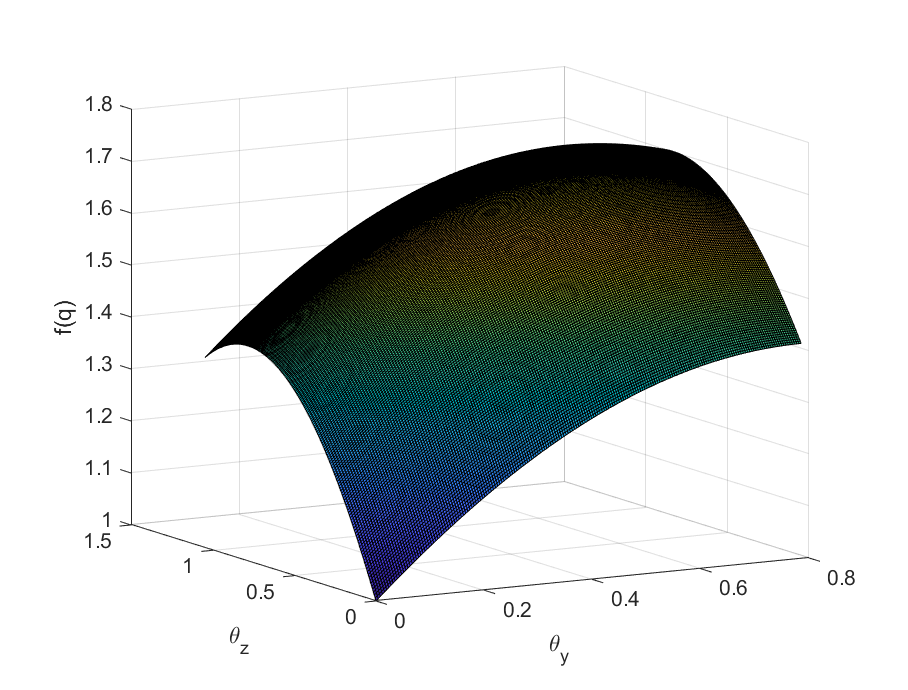
\includegraphics[width=1\linewidth]{figures/perp_area.eps}
	\caption{Perpendicular area in function of rotations around y and z axes}
	\label{fig:perp_area}
\end{figure} 
The quaternion for the minimum drag force is defined by the rotations $\theta_y = \theta_z = 0$ and the quaternion that give the maximum drag force is defined by the rotations $\theta_{y,max} = 0.61568$ rad and $\theta_{z,max} = \frac{\pi}{4}$. \\
the path between the minimum and the maximum drag force is analyzed:
\begin{flalign}
	q = q_y \otimes q_z \\
\end{flalign}
with
\begin{flalign}
	\theta_y = \alpha \ \theta_{y,max} \\
	\theta_z = \alpha \ \theta_{z,max}
\end{flalign}
and $ \alpha \in [0,1]$. the \figref{path_alpha} shows f(q) as a function of $\alpha$.
\begin{figure}[H]
	\centering
	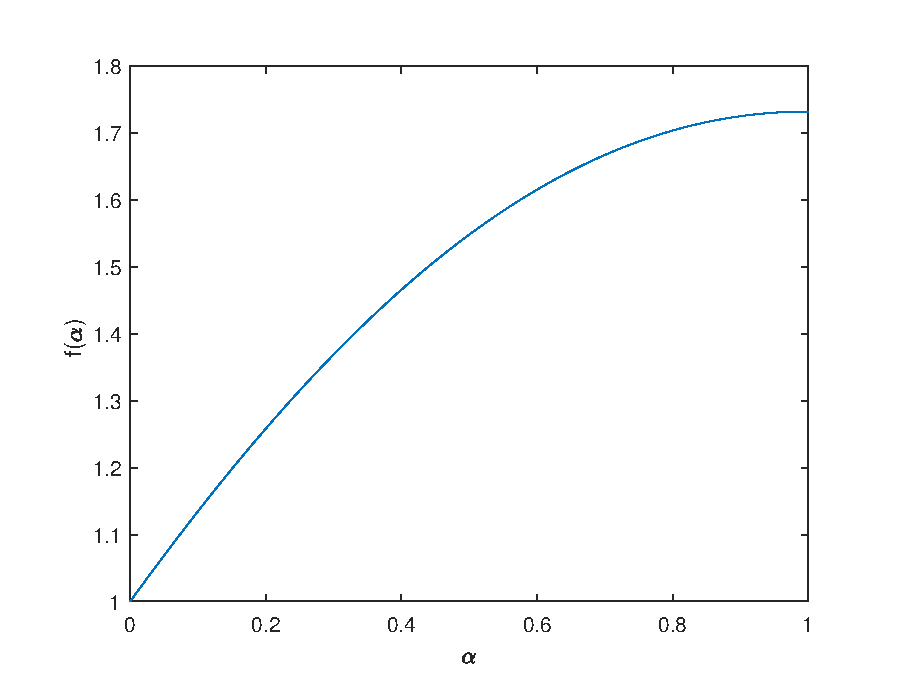
\includegraphics[width=1\linewidth]{figures/path_f.eps}
	\caption{Perpendicular area in function of rotations around y and z axes}
	\label{fig:path_alpha}
\end{figure} 
This function can be approximated by a polynomial of degree 2. the relative error of this approximation represented in the \figref{rel_err} is really small and thus, the approximation by a polynomial of degree 2 can be used. \\
\begin{figure}[H]
	\centering
	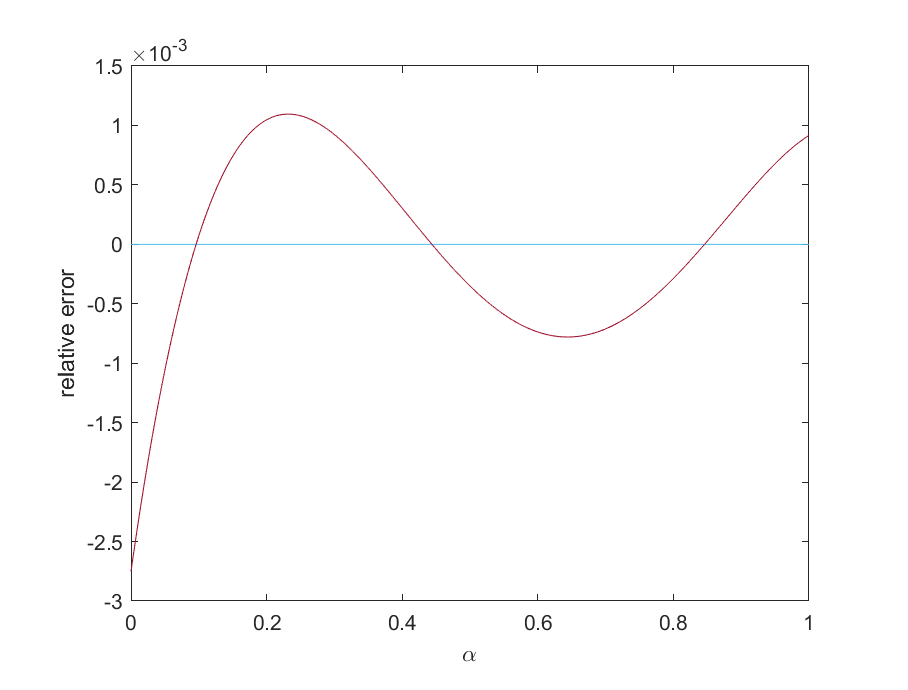
\includegraphics[width=1\linewidth]{figures/rel_err.eps}
	\caption{Relative error of the fitting approximation }
	\label{fig:rel_err}
\end{figure}
Therefore, the quaternion that give the desired drag force in the orbit frame can be computed by following this algorithm:
\begin{flalign}
	\frac{u}{u_{min}} &= f( \alpha ) \approx p_1 \alpha^2 + p_2 \alpha + p_3 \\
	\Rightarrow \alpha &= \frac{-p_2 + \sqrt{p_2^2 - 4 p_1 p_2}}{2 p_1} \\
	\Rightarrow \theta_y &= \alpha \theta_{y,max} \\
	\theta_z &= \alpha \theta_{z,max} \\
	\Rightarrow q_y &= sin(\frac{\theta_y}{2})*j + cos(\frac{\theta_y}{2}) \\
	q_z &= sin(\frac{\theta_z}{2})*k + cos(\frac{\theta_z}{2}) \\
	\Rightarrow q_{ref} &= q_y \otimes q_z
\end{flalign}
\paragraph{Nota Bene:}
This is one solution of the problem but there is an infinity of quaternions for one drag force. A better solution would be to choose the reference quaternion that give the desired drag force and that requires the smallest rotation relative to the current position of the satellite. However, this solution is very hard to implemented and we didn't find a way to do it. (i don't know if it's a good idea to say that)
\subsection{State Feedback Control}
The linearized equation \eqref{le} of the attitude system allows to design a state feedback control. However, the nominal values of the quaternion and of the angular velocity depends of the drag force desired and thus, they aren't constant all over the time. Therefore, the designed control have to stabilize the system for all the possibilities of $\bar{q}$ and $\bar{\omega}$. \\

The norm of $\bar{\omega}$ is known and to the angular velocity of the satellite around the Earth ($||\bar{\omega}|| \approx 0.0011$). Due to this value is very small compare to $\frac{1}{2}$. The A matrix can be approximated by:

\begin{flalign}
\underline{A}
\approx
\begin{bmatrix}
\underline{0}_{(3\times3)} & \frac{1}{2} \underline{\vec 1}_{(3\times3)} \\ \underline{0}_{(3\times3)} & \underline{0}_{(3\times3)}
\end{bmatrix} 
\label{eq:state_feedback}
\end{flalign} 
The system can be split in three subsystems defined by the matrix equation:

\begin{flalign}
\begin{bmatrix}
\vec{ \dot {\tilde{q}}_i(t) } \\
 \dot {\tilde{\omega}}_i(t)
\end{bmatrix} 	
= 
\begin{bmatrix}
0 &	\frac{1}{2}  \\
0 & 0	
\end{bmatrix} 
\begin{bmatrix}
\vec{  {\tilde{q}}_i(t) } \\
 {\tilde{\omega}}_i(t)
\end{bmatrix} 	
+
\begin{bmatrix}
0 \\
{I_{i,s}^{-1}}
\end{bmatrix} 	
 N_{i,c}(t)
\label{eq:le_bis}
\end{flalign}
The input control torque is defined by a state feedback law:
\begin{flalign}
Nc = 
-\begin{bmatrix}
k_1 & k_2
\end{bmatrix} 
\begin{bmatrix}
\vec{  {\tilde{q}}_i(t) } \\
{\tilde{\omega}}_i(t)
\end{bmatrix}
\end{flalign} 
Therefore, 
\begin{flalign}
A-BK = 
\begin{bmatrix}
0 & \frac{1}{2} \\
-\frac{k_1}{I_{i,s}} & -\frac{k_2}{I_{i,s}}
\end{bmatrix}
\end{flalign}
Pole Placement:
\begin{flalign}
det(sI-(A -BK)) = s^2 + \frac{k_2}{I_{i,s}} s + \frac{k_1}{2I_{i,s}}
\end{flalign} 
By Identification with a general second order equation $s^2 + 2\zeta \omega_n s + \omega_n^2$ where $\zeta$ is the damping factor and $\omega_n$ is the natural frequency, the gains are given by:
\begin{flalign}
k_1 &= -2 \ I_{i,s} \ \omega_n^2 \\
k_2 &= -2 \ I_{i,s} \ \zeta \ \omega_n
\end{flalign}
The damping factor is chosen to be equal to 1 and the rise time is chosen to be equal to 60 and thus $\omega_n = \frac{2\pi}{T_n} = \frac{2\pi}{60/0.35}$. Therefore, all the eigen values are equal to -0.0367.
\subsection{Stability}
The stability of control designed in the previous section have to be checked for all $\bar{\omega}$. Due to the fact that the matrix A is affine in $\bar{\omega}$. The stability can be only checked on the vertices of the convex polyhedron (cube) that contains all the possibilities of $\bar{\omega}$ as represented in the \figref{sta_PID} (reference lectures NLCS).
\begin{figure}[H]
	\centering
	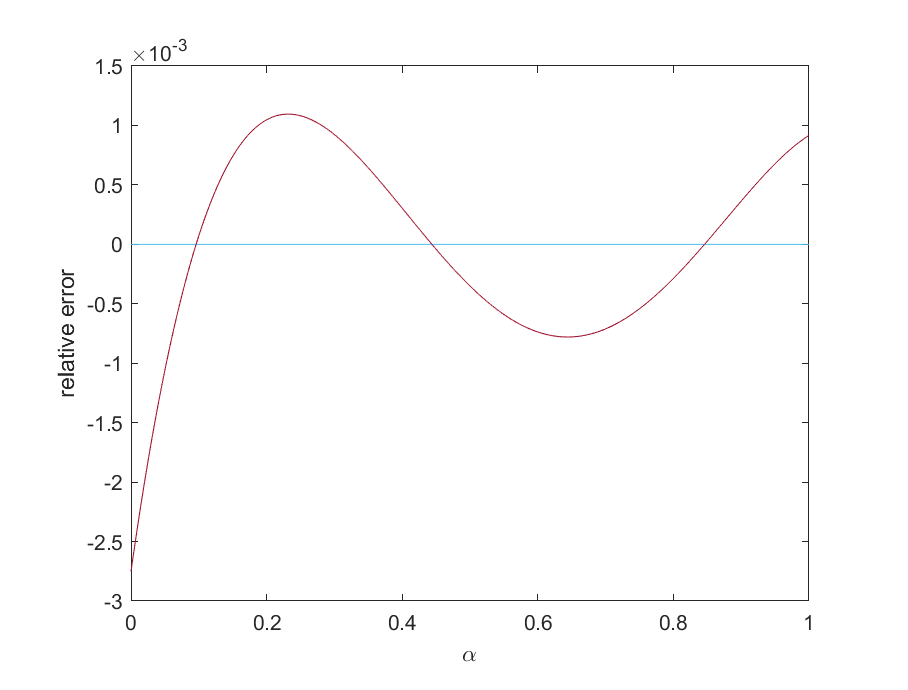
\includegraphics[width=1\linewidth]{figures/rel_err.eps}
	\caption{Convex Polyhedron}
	\label{fig:sta_PID}
\end{figure} 
The maximum real part of the eigenvalue in the vertices of the cube is equal -0.0308 that is very close to the desired eigenvalue.